\documentclass[twoside, a4paper, DIV=11,twocolumn]{book}
% \documentclass[oneside, a4paper, DIV=11]{book}

% PACKAGES
\usepackage[ngerman]{babel}
\usepackage[utf8]{inputenc}
\usepackage[singlespacing]{setspace} % 1,5 Zeilenabstand: onehalfspacing
\usepackage[nottoc]{tocbibind} % Literaturverzeichnis im Inhaltsverzeichnis
%\usepackage{subscript} % Tiefegestellter Text außerhalb des Mathemodus
\usepackage{fixltx2e} % Tiefegestellter Text außerhalb des Mathemodus
\usepackage{amsmath,
	    amssymb,
	    array,
	    balance, % gleich lange säulen am ende jedes Kapitels
	    color,
	    graphicx,
	    hyphsubst, % Silbentrennung wie ich es will
	    hyperref,
	    natbib,
	    ragged2e,
	    sectsty,
	    siunitx, 
	    tabularx,
	    tikz}

% \usepackage{pdflscape,}
%\hypersetup{linktocpage} % nur die Seitenzahlen erscheinen als Link
\usepackage{./src/mymacros}
\usepackage{./docu/bscmakros}

\usepackage{etoolbox} % citations in italic:
\makeatletter
\patchcmd{\NAT@test}{\else\NAT@nm}{\else\NAT@nmfmt{\NAT@nm}}{}{}
\let\NAT@up\itshape
\makeatother


% \usepackage{showframe} % show margins and stuff

% SETTINGS

\hypersetup{
    colorlinks,
    citecolor=black,
    filecolor=black,
    linkcolor=black,
    urlcolor=black
}

\sisetup{
    locale=DE,
    loctolang={DE:ngerman},
    load-configurations = binary,
    binary-units = true,
    list-final-separator = { \translate{und} },
    list-units=single,
    range-phrase = { \translate{bis} },
    range-units=single,
    round-mode = places,
    round-precision = 3
}

\pagestyle{plain}

% sectsty setup
\chapterfont{\raggedright}
\sectionfont{\raggedright}

%TITLE
\title{Transport durch Dichteinstabilitäten in einer Hele-Shaw Zelle}
\author{Johannes Haux}
\date{1.4.2015}

%DOCUMENT
\begin{document}

\onecolumn
\begin{titlepage}
\begin{center}
 
\Large\textbf{Department of Physics and Astronomy\\
University of Heidelberg}

\vspace{16cm}

\normalsize
Bachelor Thesis in Physics\\
submitted by \\
\vspace{0.5cm}
\Large\textbf{Johannes Stefan Jacob Haux}\\
\normalsize
\vspace{0.5cm}
born 1989 in Tübingen (Germany)\\
\vspace{0.5cm}
\Large\textbf{2015}
\normalsize

\pagenumbering{gobble}% Remove page numbers (and reset to 1)
\clearpage
\thispagestyle{empty}

\newpage
\mbox{\,}
\newpage
\pagenumbering{gobble}% Remove page numbers (and reset to 1)
\clearpage
\thispagestyle{empty}

\mbox{\,}

\vspace{2.5cm}

\Huge
\onehalfspacing

\textbf{Transport durch \COTm induzierte Dichteinstabilitäten in einer \HSC}

\normalsize
\singlespacing

\vspace{3cm}

% Johannes Haux
% 
% 2015


\vspace{7.5cm}

\normalsize
This Bachelor Thesis has been carried out by Johannes Stefan Jacob Haux at the\\
Institute of Environmental Physics in Heidelberg\\
under the supervision of\\
Prof. Dr. Kurt Roth

\vfill
\end{center}
\newpage
\mbox{\,}
\newpage
\end{titlepage}

\clearpage
\pagenumbering{arabic} % von der Uni gefordert. ggf anpassen

\emptypage

% Zusammenfassungen
\newpage
\pagenumbering{roman}

% \maketitle
\chapter*{\,}

 %Deutsch
  \noindent \textbf{Zusammenfassung} \hspace{0.3cm} In dieser Arbeit wird der Einfluss von dichtegetriebenen Instabilitäten gezeigt, welche durch das Lösen von \COT an der Wasseroberfläche in einer \HSC herbeigeführt werden. 
  Mit Hilfe eines pH-Indikators und einer optischen Methode kann die Ausbreitung des \COT räumlich und zeitlich aufgelöst und untersucht werden. 
  Es werden qualitativ drei Phasen im Verlauf des Experiments festgestellt, in denen je ein anderer Prozess (Diffusion, stabile Fingerentwicklung, Vortizität auf Zellebene) dominiert und zudem charakteristische Längen und Zeiten der Fingerbildung bestimmt, welche durch die Instabilitäten ausgelöst wird und konvektiv das \COT in tiefere Wasserschichten transportiert.
  Eine Analyse der Methoden zeigt, wie durch erweiterte Experimente eine detaillierte quantitative Auswertung ermöglicht werden könnte.
  
  Eine einfache Übertragung des Experiments auf eine heterogen gefüllte \HSC ist nicht möglich. Die notwendigen Schritte zum Erreichen dieses Ziels werden diskutiert.
  
  \vspace{1.5cm}
 
 %Englisch
  \noindent \textbf{Abstract} \hspace{0.3cm} In this thesis the influence of density driven instabilities are investigated. These instabilities are induced experimentally by solving \COTm gas into water through the air/water interface on top of the water, inside a Hele-Shaw cell. 
  Using a pH-sensitive indicator and an optical method, the propagation of \COT is analysed spatially and over time.
  The experiment is found to be characterized qualitatively by three phases with different dominating processes (diffusion, stable finger evolution and cell scale vorticity). Additionally the characteristic length- and timescales of the second phase of stable finger evolution are determined. This phase is caused by the instabilities and transports water convectivly into deeper water layers. 
  An analysis of the methods used shows, how enhanced experiments could facilitate a more detailed and quantitative evaluation. 
  
  At the end, possibilities for executing the experiment in a heterogeniously filled Hele-Shaw cell are discussed.

\emptypage

\tableofcontents

\emptypage

\listoffigures

\newpage

% jetzt gehts los
\pagenumbering{arabic}
\twocolumn
\balance % gleich lange säulen am ende jedes Kapitels
\chapter{Einleitung}

% Gutes Verständis, da Bodenphysik immer gute Beisiele hat:
% Salzsee, CO2 einlagerung
\label{sec:intro}

Während der Durchführung meiner Bachelorarbeit entstanden zunächst Ideen zu einem Experiment, dass sich schließlich als nicht durchführbar herausstellte, für den zur Verfügung stehenden Zeitraum. In Folge dessen kam die Idee zu einem weiteren, für die zur Verfügung stehende Zeit besser geeignetem Experiment. Aus diesem Grund teiltsich diese Arbeit in jedem ihrer Abschnitte immer in inhaltlich dem einen, wie dem anderen Experiment zugehörigen Bereiche.

Grundlegend für alle Fragestellungen, die im Laufe dieser Arbeit aufkamen, sind Dichteinstabilitäten, die zur treibenden Kraft von Prozessen werden, die mit Hilfe einer Hele-Shaw-Zelle beobachtet werden sollen.
Zunächst wird die Frage gestellt, wie sich Verdunstungsphänomene auf Stofftransport in gesättigten, heterogenen, porösen Medien auswirken und zu Stofftransport von der Oberfläche in tiefere Schichten führt. Als Beispiel kann man sich einen Salzsee vorstellen, der dabei ist auszutrocknen und dabei Salz in tiefere Erdschichten einlagert.
In einem zweiten Ansatz wird die Frage gestellt, wie sich in Wasser lösendes \COT für Dichteinstabilitäten sorgt, die schließlich das gelöste Gas in tiefer Wasserbereiche führt. Auch hier lässt sich wieder ein sehr Anwendungsbezogenes Beispiel finden, wie schon \cite{fernandez} treffend festgestellt hat: Das Einlagern von \COT in Gesteinsschichten setzt vorraus, dass sich das \COT lange genug auf dem Gestein aufhält. Sorgt man dafür, dass unterirdische Wasserreservoirs mit \COT gesättigt werden kann man dieses Verhalten künstlich herbeiführen. Ein Verständnis dafür, wie sich \COT in Wasser löst und bewegt ist dafür grundlegend.

Diese Arbeit ist gegliedert in folgende Teile: Zunächst soll in Teil \ref{sec:theo} eine theoretische Grundlage geschaffen werden, zum Verständis der folgenden Abschnitte. Anschließend erkläre die Teile \ref{sec:set} "Experimenteller Aufbau" und \ref{sec:ima} "Bildanalyse" die Methoden, mit denen Messdaten beschaffen und ausgewerted wurden. Die Ergebisse dieser Messungen werden in Teil \ref{sec:res} "Ergebnisse" präsentiert und diskutiert. 
Am Ende folgt eine Zusammenfassunge mit Ausblick.

\chapter{Grundlagen}

\label{sec:theo}
\section{Poröse Medien}
\label{theo:por}

\TODO{porosität + leitfähigkeit}
\section{Fingerbildung}
\label{theo:fing}

\chapter{Experimenteller Aufbau}

\label{sec:set}

Da für beide in Teil \ref{sec:intro} beschriebenen Fragestellungen die Dynamik der betrachteten Systeme interessant ist, wird jeweils ein ``Light Transmission Experiment''
durchgeführt. Hierzu wird eine Hele-Shaw Zelle vor einer homogenen Lichtquelle plaziert. Das Licht, dass die Zelle durchdringt wird anschließend von einer Digitalkamera aufgezeichnet
und für die spätere Auswertung gespeichert.
Größter Unterschied bei den Experimenten ist vor Allem die Dauer. Während das Verdunstungsexperiment fast zwei Wochen dauert ist das \COT-Experiment auf maximal wenige Stunden ausgelegt. 
\TODO{muss der letzte Satz sein?}
\widegraph[./plot/Aufb_Dunst.png]{Grundsätzlicher Aufbau der beiden durchgeführten Experimente. Zu sehen sind: 1: Lichtquelle, 2: Hele-Shaw-Zelle, 3: Kamera \TODO{Beschriftung und passendes Bild}}{fig:auf}

\section{Hele-Shaw Zelle}
\label{sec:hsc}
Grundsätzlich besteht die Hele-Shaw Zelle aus zwei Glasplatten, die einem kleinen Abstand zueinander gehalten werden. Bei diesem Aufbau sind drei der vier Seiten abgedichtet, sodass kein Wasser abfließen kann. 
Die offene Seite der Zelle zeigt nach oben. Auf diese Weise soll dafür gesorgt werden, dass die auftreten Strömungseffekte annähernd zweidimensional sind. 
\TODO{schönere Formulierung}, \TODO{Beleg!}
Die Abmessungen der verwendeten Zellen sind in Tabelle \ref{tab:Hdim} festgehalten.
Am unteren Ende der Zelle befindet sich ein Ausfluss, über den die Zelle kontroliert mit Wasser oder einer gewünschten Lösung befüllt werden kann.


\inkscape{./plot/cell_dimensions.pdf_tex}{\linewidth}{Dimensionierung der Hele-Shaw Zelle. Ansicht von oben und von der Seite. 1:Keil, 2: Dichtung und Abstandshalter, 3: Rahmen, 4: Glasplatte, 5: Füllung der Zelle.}{fig:Hdim}

\begin{table}[h]
  \begin{tabular}{p{2cm}|c|c|c}
    Aufbau			& Höhe				& Breite			& Abstand \\
    \hline\hline
    Verdunstungs\-experiment	& \SI{ 500}{\milli\meter}	& \SI{273}{\milli\meter}	& \SI{3}{\milli\meter} \\
    \COT-Experiment		& \SI{ 250}{\milli\meter}	& \SI{273}{\milli\meter}	& \SI{2,1}{\milli\meter}  
  \end{tabular}
  \caption{Dimensionierung der Hele-Shaw Zellen für die beiden durchgeführten Experimente. Siehe auch Abbildung \ref{fig:Hdim}.}
  \label{tab:Hdim}
\end{table}


\section{Kamera}
\label{sec:cam}
Die Messung wird mit Hilfe einer Kamera durchgeführt. \TODO{Modell, Objektiv}. Der Sensor des benutzten Modells zeichnet sich durch seine stark linearen Eigenschaften aus, wie schon bei \cite{buchner}

\section{Lichtquelle}
\label{sec:light}


\section{Das Verdunstungsexperiment}
\label{set:eva}

Hier kommt eine KURZE Beschreibung des Verdunstungsexperiments hin!

\graph{Aufbau des Verdunstungsexperiments. Zu Sehen sind 1. , 2. , ...}{gr:suevp}
Für das Verdunstungsexperiment wird die Hele-Shaw Zelle mit Glasküglechen verschiedener Größen gefüllt. Dabei wurde darauf geachtet, dass die immer homogene Regionen enstehen. Die Größen der verwendeten Kugeln der Firma Sili-Beads\TODO{Referenz und Tabelle und tm Logo oder so} sind in Tabelle \ref{ref:kug} notiert. Die Porosität
dieser Regionen kann über die Radien der Kügelchen abgeschätzt werden, wie es auch bei \cite{feustel} gemacht wurde. \TODO{original quelle finden und verwenden}
Wie in Teil \ref{theo:por} beschrieben, führen damit die Kugelgrößen zu verschiedenen Leitfähigkeiten. Auch diese sind in Tabelle \ref{tab:kug} festgehalten.
Eine sehr genaue Beschreibung des Aufbaus kann bei \cite{buchner,heberle} nachgelesen werden.


\section{Das \COT-Experiment}
\label{set:cot}
%\subsubsection{\(\COT Experiment in porous media\)}
%\label{set:cpm}


\chapter{Methoden}
\label{cha:meth}

Alle durchgeführten Experimente wurden, wie in Kapitel \ref{cha:set} beschrieben, mit Hilfe einer Kamera aufgezeichnet. Die Auswertung beruht daher in einem 
ersten Schritt darin die gewünschten Informationen aus den Bildern zu gewinnen. In allen durchgeführten Experimenten ist dies die Verfolgung eines Tracers, 
welcher andere Absorptionseigenschaften hat, als das ihn umgebende Material.
In einem nächsten Schritt werden die so gewonnen Daten genommen und weiter ausgewertet, um Informationen über das Verhalten der Beobachteten Phänomene zu 
erhalten.

Im Folgenden werden häufig die Begriffe ``Helligkeit'', ``Grauwert'' und ``Intensität'' synonym verwendet. Sie bezeichnen alle die selbe Information: Den 
Grauwert \TODO{$i \geq 0$} eines Pixels, bzw. die Grauwerte eines Pixelarrays.

\section{Bildanalyse}
\label{sec:ima}
% verwendete Software
Die vorgenommenen Bildanalysen wurden mit Hilfe von \cite{python} (Version 2.7) durchgeführt. 
% Hauptsächlich wurden die Pakete OpenCV (Version 2, zum Laden der Bilder), numpy (Verarbeitung der Bilder, Matrixoperationen) und matplotlib (Darstellung/Speichern und Plotten) verwendet.
% Einlesen der Bilder
Ein Bild, welches von OpenCV eingelesen wird besteht aus drei \SI{8}{\bit} Kanälen. Da die Kamera aber ein monochromes Bild aufgezeichnet hat, ist davon 
auszugehen, dass das eigentlich einkanalige Bild künstlich auf drei Kanäle umgerechnet wurde. Der Einfachheit halber wird über die Kanäle gemittelt und man 
erhält ein Array aus Grauwerten mit dem weiter gerechnet wird.

% Differenzen Methode
Zur Bestimmung der Position eines Tracers stehen verschiedene Möglichkeiten zu Verfügung.
Unter der Annahme, dass die aufgezeichneten Bilder $\mathbf{B}$ zu allen Zeiten in allen Bereichen gleich belichtet sind, kann man ein Referenzbild $\mathbf{R}$ 
vom Rest der Bilder abziehen. Als Referenz wird das erste Bild der Messung, bei noch unverändertem Ausgangszustand gewählt.
Als Ergebnis erhält man Matrizen $\mathbf{C}$, welche in unveränderten Bereichen den Wert Null annehmen, ansonsten aber ungleich null sind:
\begin{eqnarray}
 \mathbf{C} = \mathbf{B} - \mathbf{R}
\end{eqnarray}


Allerdings lässt sich leicht feststellen, dass die aufgezeichneten Bilder in ihrer Helligkeit schwanken. Bilder die früher aufgezeichnet wurden sind heller, als 
solche, die später gemacht wurden. Um diesem Effekt entgegenzuwirken wird ein Algorithmus implementiert, der einen Bildbereich betrachtet, dessen Helligkeit 
während der gesamten Messung konstant bleiben sollte. Sei $\mathbf{B}$ ein beliebiges Bild der Messreihe und $\mathbf{R}$ das Referenzbild. Dann sind 
$\mathrm{M(\mathbf{B})}$ und $\mathrm{M(\mathbf{R})}$ die Arrays aus $N$ Pixeln, die den Bildbereich mit konstanter Intensität beschreiben. Aus allen Elementen 
wird der jeweilige Mittelwert dieser beiden Matrizen errechnet:
\begin{eqnarray}
 \mu_{\mathbf{B}} = \frac{1}{N} \sum_{i=1}^N \mathrm{M(\mathbf{B})}_i \\
 \mu_{\mathbf{R}} = \frac{1}{N} \sum_{i=1}^N \mathrm{M(\mathbf{R})}_i
\end{eqnarray}

Aus diesen Werten lässt sich nun ein Faktor $f$ zur Korrektur des Bildes errechnen, da gilt:
\begin{eqnarray}
 \mu_{\mathbf{R}} = f \cdot \mu_{\mathbf{B}}
\end{eqnarray}

Damit lassen sich alle Grauwerte des Bildes auf den passenden Wert korrigieren ($\mathbf{B}_{neu} = f \cdot \mathbf{B}$) und man erhält einen neuen Wert für die 
Differenzmatrix:
\begin{eqnarray}
 \mathbf{C} = f \cdot \mathbf{B} - \mathbf{R}
 \label{eq:norm}
\end{eqnarray}


% Quotientenmethode
Neben der schwankenden Helligkeit fällt auch noch auf, dass die LED-Beleuchtung zu einer Vignettierung der Aufnahme führt, da die Beleuchtung in der Mitte 
stärker als an den Rändern. Ein einfaches Substrahieren der Bilder führt also zu einer Unterschätzung der absoluten Grauwerte im Außenbereich, bzw. zu einer 
Überschätzung im Innenbereich des Bildes.
Unter der Annahme, dass diese Vignettierung über den Zeitraum der Messung konstant bleibt, wird anstelle der Subtraktion eine Division durchgeführt, \dah jedes 
Pixel $\mathbf{b}_{nm}$ des untersuchten Bildes wird durch das Pixel $\mathbf{r}_{nm}$ des Referenzbildes an selber Stelle geteilt, wobei gilt 
$\mathbf{B} = \mathbf{b}_{nm}$ und $\mathbf{R} = \mathbf{r}_{nm}$. Zusammen mit Gleichung \ref{eq:norm} erhält man folgende Bildungsvorschrift für die 
Quotientenbilder:
\begin{eqnarray}
 \mathbf{C} = \mathbf{c}_{nm} = \frac{f * \mathbf{b}_{nm}}{\mathbf{r}_{nm}}
 \label{eq:quot}
\end{eqnarray}
Die Werte von $\mathbf{C}$ nehmen den Wert 1 überall dort an, wo Referenz- und betrachtetes Bild gleich sind. Der Tracer befindet sich also dort, wo gilt 
$\mathbf{c}_{nm} \neq 1$.

Zur leichteren Interpretation werden die Werte vor der graphischen Visualisierung auf einen Wertebereich von 0 bis 100 normiert.

\section{Detektion und Verfolgung des Tracers im Fall von Fingerbildung}
\label{sec:track}
Während der \COT-Experimente wird beobachtet, dass sich herabsinkende Finger der Wasser-\COT-Lösung, bilden. Deren Position und Länge über den Zeitraum der 
Messung, bzw. der ersten Minuten, sind interessante Größen, die dabei helfen können, das System zu beschreiben und zu verstehen.

Wird im folgenden von ``Bild'' gesprochen, so ist vom Quotientenbild nach Gleichung \ref{eq:quot} die Rede. Mit anderen Worten bezeichnet ``Bild'' die räumlich 
aufgelöste Tracerkonzentration zu einem bestimmten Zeitpunkt der Messung.

\subsection{Detektion}
\label{sec:dec}
Zunächst wird ein Bereich des zu untersuchenden Bildes festgelegt, in dem sich nur Indikatorflüssigkeit befindet. Nach Möglichkeit schließt die obere Kante 
dieses Bildbereiches genau mit der Wasserkante ab. Ein Herausragen über die Wasserkante wird vermieden, da die Hintergrundbeleuchtung für sehr helle 
Intensitätswerte sorgt. Da auch die Finger für höhere Intensitäten sorgen (siehe Teil \ref{sec:cot}) würde sonst die Messung systematisch beeinflusst. Der 
Bereich bleibt für alle Bilder gleich.

Aus dem so erhaltenen Array $\mathbf{C} = \mathbf{c}_{nm}$ ($n \in 1,\dots,N$ und $m \in 1,\dots,M$) wird von jeder Säule der Mittelwert berechnet. Man erhält 
ein Array der mittleren, vertikalen Intensitäten $\mathbf{I} = \mathbf{i}_{n}$:
\begin{eqnarray}
 \mathbf{i}_{n} = \frac{1}{M} \sum_{i=1}^{M} \mathbf{c}_{ni}
\end{eqnarray}

Für jedes Bild, bzw. jeden Zeitschritt erhält man so ein charakteristisches Signal. Unter der Annahme, dass die Finger sich gerade nach unten bewegen, befindet 
sich ein Finger an jedem lokalen Maximum von $\mathbf{I}$. Über die Richtigkeit dieser Annahme wird in Teil \ref{res:cot} diskutiert.
Da das Signal verrauscht ist wird eine diskrete Fourieranalyse durchgeführt, um das Wellenzahlenspektrum zu erhalten. So kann analysiert werden, in welchen 
Abständen Finger vorwiegend auftreten. Bereinigt man dieses Spektrum von den Werten, die dem Rauschen zugeordnet werden und führt eine Rücktransformation in den 
ursprünglichen Raum durch, kann man genau sehen, wo sich die Intensitäts-Maxima befinden. Wiederholt man dieses Verfahren zu jedem Zeitschritt erhält man eine 
zeitaufgelöste Vorstellung davon, wo sich die Finger im Verlauf des Experiments befinden.

\TODO{==========}
\subsection{Länge}
\label{sec:lan}
Mit dem Wissen, wo sich die Finger befinden, lässt sich auch deren Länge errechnen. Dazu wird an jeder Stelle $s$ im Array $\mathbf{C}$ aus Teil \ref{sec:dec}, 
wo sich ein Finger befindet, die Pixelsäule $\mathbf{c}_{sm}$ von unten nach oben abgewandert ($m \in M, \dots, 1$), bis ein Schwellenwert $c_{crit}$ 
überschritten ist, der festlegt, ab welchem Grauwert von einem Finger die Rede ist. Um dieses Wert nicht durch Rauschen zu früh zu detektieren, wird über eine 
Reihe von 5 Pixeln links und rechts von $\mathbf{c}_{sm}$ gemittelt. Der so erhaltene Wert für $m(c_{crit})$ gibt die Länge $l$ des Fingers in Pixeln an.
\begin{align}
 m &\in (M,\dots,1) \\
 l(m) &= \left(\frac{1}{10}\sum_{i=s-5}^{s+5} \mathbf{c}_{im} \leq c_{crit} \right) \, ? \; l(m-1) : m \\
 l(0) &= 0
\end{align}

In Abbildung \ref{fig:f_detect} und \ref{fig:fgrowth} sind Beispiele für die Detektion und bestimmte Länge der Finger zu finden.

\subsection{Wachstum}
\label{sec:grow}
Mit der Annahme, dass alle Finger gleich schnell wachsen, reicht es aus, zu jedem Zeitschritt $t_i$ den Mittelwert $\bar{l}_i$ der Länge aller Finger zu 
berechnen und anschließend durch den Zeitschritt zu teilen, um ihre Wachstumsrate zu ermitteln. 
\begin{align}
 \dot{l}_i &= \frac{\bar{l}_i-\bar{l}_{i-1}}{t_i-t_{i-1}} \\
 i &\in \mathbb{N} \\
 \bar{l}_{0} &= 0
\end{align}
man aber beobachten kann, dass die Finger in unterschiedlichen Bereichen unterschiedlich schnell wachsen, wird eine Methode implementiert, die es erlaubt, Teile 
des untersuchten Arrays $\mathbf{C}$ zu betrachten. Das bedeutet, es werden nur die Längen der Finger in diesem Bereich in Betracht gezogen. Wählt man den 
Bereich klein genug ist es möglich auch einzelne Finger zu betrachten.

\TODO{raus? ======}

\chapter{Ergebnisse}

\label{cha:res}
% \section{Verdunstungsexperiment}
% \label{res:eva}
% 
% \subsection{Präsentation}
% \label{res:eva:pres}
% 
% \widegraph[./plot/plot_eva]{Das Verdunstungsexperiment (a) zu Beginn der Messung und (b) am Ende nach 16 Tagen und 1,5 Stunden. Die Aufnahmen enstanden in Kombination mit einem \SI{630}{\nano\meter}-Filter. Die Ausbreitung den \BB Tracers ist mit einer weißen gestrichelten Linie bei (b) und (c) eingezeichnet. (c) Zeigt die Differenz der beiden Bilder (siehe Teil \ref{sec:ima}), normiert auf den Wertebereich $(0,\dots,100)$. Man kann erkennen, dass die Zelle im Verlauf der Messung gekippt ist (rote und blaue Streifen im oberen Teil des Bildes).}{fig:reseva}
% 
% 
% Das Verdunstungsexperiment wurde über einen Zeitraum von 16 Tagen und 1,5 Stunden durchgeführt. In Abbildung \ref{fig:reseva} kann man das Ergebnis der Messung sehen. Klar zu erkennen ist, dass sich der \BB-Tracer weit nach oben ausgebreitet hat, ca. über die Hälfte der Zelle. Bevorzugt wurde dabei der Weg über die Mitte der Zelle, was an der keilartigen struktur der Tracerausbreitung ausgemacht wird. 
% 
% Mit Hilfe der Differenzenmethode aus Teil \ref{sec:ima} und durch betrachten der Abfolge aller aufgenommener Bilder in Form eines Films, lässt sich erkennen, dass die Zelle über den Zeitraum des Experiments leicht nach vorne gekippt ist. Dadurch bilden sich rote und blaue Linien aus, da die flaschen Regieonen voneinander abgezogen werden. Eine Abschätzung, wie der Tracer sich ausgebreitet hat ist dennoch in Kombination mit der Originalaufnahme sehr gut möglich und reicht für die qualitative Abschätzung, wie sie hier erfolgen soll.
% 
% 
% \subsection{Schlussfolgerungen}
% \label{res:eva:disk}
% 
% Eine sehr grobe Abschätzung der Menge, des verdunsteten Wassers kann über die Fläche, die der Tracer einnimmt gemacht werden. So wie sie hier durchgeführt wird, kann und soll sie keine harten wissenschaftlichen Daten liefern, aber in Zahlen fassen, was man intuitiv sieht.
% 
% Unter der Annahme, dass die Kügelchen in der Zelle so dicht wie möglich gepackt sind ist die Porosität an allen Stellen $\bar{\phi} = 0,35$. Diese Annahme stellt natürlich eine untere Grenze dar, da die Kugeln nicht perfekt liegen. 
% Die eingenommene Fläche wird mit $\frac{1}{3}$ der Zellenfläche abgeschätzt. Zusammen mit den Abmessungen der Zelle (Tabelle \ref{tab:hsc}) erhält man das abgeschätzte Volumen $V_w$ des verdunsteten Wassers:
% \begin{align}
%  V_{HS-Zelle} &=  \SI{0,4095}{\liter} \\
%  \Rightarrow V_{w} &= \frac{\bar{\phi}}{3} \cdot V_{HS-Zelle} = \SI{0,04778}{\liter}
% \end{align}
% Teilt man dieses Ergebnis durch die Zeitdauer des Experiments erhält man eine Abschätzung für die Verdunstungsrate:
% \begin{align}
%  \dot{V_w} = \SI{0.1239}{\milli\liter\per\hour}
% \end{align}
% 
% \TODO{Vergleich Arbeit Apple}



% \newpage
\section{\COTm Experiment}
\label{res:cot}

\sisetup{
  round-mode=places,
  round-precision=1
}


% ========================= Allgemeiner Verlauf =========================
In den Abbildungen \ref{fig:fft} bis \ref{fig:complete} sind die Ergebnisse des \COTm Experiments festgehalten. Die Gesamtdauer des Experiments beläuft sich auf \mbox{\SI{5}{\hour} \SI{6}{\minute}}, der für diese Arbeit interessante Übergang zur Fingerbildung findet nach \SI{9}{\minute} statt. Nach ca. \SI{1,5}{\hour} wird das Verhalten zunehmend von Konvektion auf Zellskala dominiert, weshalb spätestens hier alle in Teil \ref{cha:meth} beschriebenen Methoden versagen. 
Die Konvektion auf Zellskala sorgt für Durchmischung indem die Finger nicht mehr gerade nach unten sinken können, sondern zur Seite driften, wo sie wieder nach oben gedrückt werden.

Wie erwartet kann sehr gut die Fingerbildung beobachtet werden. Abbildungen \ref{fig:vcot_1-1}, \ref{fig:vcot_1-2} und \ref{fig:vcot_1-grey} zeigen ihren zeitlichen Verlauf.


% ========================= fft & k_space =========================
\widegraph[./plot/plots_data-1/fft]{Die mit Hilfe der diskreten Fourieranalyse vom Rauschen bereinigten mittleren Intensitäten der Finger. Der zeitliche Verlauf ist farblich codiert und geht von \SI{0}{\minute} (hellblau) bis \mbox{\SI{1}{\hour} \SI{24}{\minute}} (pink).}{fig:fft}

\graph[./plot/plots_data-1/k_space]{Mit Hilfe der diskreten Fourieranalyse bestimmte Abstände (hier in der Einheit $\si{Finger \per \centi\meter}$) der Finger. Man kann gut erkennen, dass dieser bei $k \approx \SI[round-precision=2]{0,66}{\per\centi\meter}$ liegt. Der zeitliche Verlauf ist farblich codiert und geht von \SI{0}{\minute} (hellblau) bis \mbox{\SI{1}{\hour} \SI{24}{\minute}} (pink).}{fig:k_space}

Zur Fingerdetektion wurde, wie beschrieben, eine Fourieranalyse der mittleren Wellenintensitäten gemacht (siehe Teil \ref{sec:dec}). Die resultierenden Spektren der Wellenzahlen $k(t)$ sind in Abbildung \ref{fig:k_space} zu sehen. Hier kann man erkennen, dass über den ersten Zeitbereich des Experiments zwischen \SIrange{9}{50}{\minute}, ein Abstand von \SI[round-precision=2]{1,517}{\centi\meter} ($\Rightarrow k=\SI[round-precision=2]{0,66}{\per\centi\meter}$) zwischen den Fingern dominiert und im zeitlichen Verlauf stabil bleibt. 

Der zeitliche Verlauf der mit Hilfe dieser Fourieranalyse bereinigten, mittleren Fingerintensitäten ist in Abbildung \ref{fig:fft} dargestellt. Es wurden alle Signale mit einer Wellenzahl $k > \SI{2}{\per\centi\meter}$ als Rauschen eingestuft und ausgefiltert. Hier kann man gut das Wachstum der Finger, in Form der steigenden Amplitude, erkennen, sowie die Bewegung der Finger. %, die relativ konstant bleibt. 

% ========================= Fingerzahl =========================
% \graph[./plot/plots_data-1/fcount]{Anzahl der detektierten Finger im Verlauf des Experiments. Das Rauschen tritt auf, da die Methode nicht einwandfrei funktioniert. Siehe dazu auch \ref{fig:f_detect}. Im Zeitraum von \SIrange{9}{40}{\minute} liefert sie allerdings relativ verlässliche Ergebnisse.}{fig:fcount}

\graph[./plot/plots_data-1/fgrowth]{Länge der detektierten Finger im Verlauf des Experiments. Das Rauschen tritt auf, da die Methode nicht einwandfrei funktioniert. Siehe dazu auch \ref{fig:f_detect}. Im Zeitraum zwischen \SIrange{9}{40}{\minute} liefert sie allerdings relativ verlässliche Ergebnisse.}{fig:fgrowth}

% Die Graphen \ref{fig:fcount} und \ref{fig:fgrowth} zeigen Zahl und mittlere Länge der Finger über den Verlauf der Messung. 
Der Graph \ref{fig:fgrowth} zeigt die mittlere Länge der Finger im Verlauf der Messung. Für diese Betrachtung wurde der untersuchte Bereich der \HSC in 9 gleich große Teile aufgeteilt und über die Längen der Finger in diesen Bereichen gemittelt, um zu sehen, ob das Wachstum in verschiedenen Bereichen der Zelle unterschiedlich ist.
Hier zeigt sich, was auch aus  Abbildung \ref{fig:vcot_1-1} zu erkennen ist: die Länge der Finger nimmt relativ linear zu.

% einzelner Finger
Für generauere Betrachtung des Übergangs vom diffusiven zum konvektiven Vermischungsprozess von Wasser und \COT sind in Abbildung \ref{fig:vcot_1-grey} und \ref{fig:sevo} die ersten \SI{16}{\minute}, bzw. \SI{52}{\minute} des Experiments gezeigt. Hierfür wurden die originalen Aufnahmen verwendet, da man hier deutlicher den Effekt beobachten kann.

Man kann erkennen, dass im Verlauf des Experiments, zwischen \SI{5}{\minute} und \SI{9}{\minute} der Übergang stattfindet. Anschließend bilden sich zunächst schnell, ab \SI{24}{\minute} etwas langsamer Finger aus. Direkt zu Beginn der Fingerbildung kann man sehen, wie die diffusive Schicht abgesaugt wird, ebenso wie kürzere Finger. Dies wird in Abbildung \ref{fig:sevo} (\SIrange{9}{26}{\minute}) besonders deutlich. In diesem Zeitraum kann man beobachten, wie rechts und links von dem am größten hervorragenden Finger die diffusive Schicht kleiner wird, bis sie fast wieder reines Wasser an der Wasseroberfläche ist. Nach \SI{24}{\minute} ist die obere \COT Schicht wieder so dick wie nach \SI{9}{\minute}. Nach \SI{39}{\minute} sorgen Turbulenzen dafür, dass die Schicht wieder dünner und vom Finger abgeleitet wird.

Letztendlich verschmelzen immer mehr Finger miteinander und es gibt nach einer Stunde immer weniger Finger (siehe \zB Abbildung \ref{fig:complete}). Diese wandern entlang der Wasseroberfläche.
Nach \SI{5}{\hour} ist die Zelle sehr gut, wenn auch noch nicht komplett, durchmischt.


\subsection{Diskussion}
\label{res:cot:disk}

Ein Vergleich der oben gezeigten Ergebnisse mit denen aus anderen Arbeiten zeigen gute Übereinstimmungen.
\cite{kneafsy} beschreiben in Ihrer Arbeit die \COTm Sequestration, so wie sie auch hier zu beobachten ist. Auch dort wird der Effekt beobachtet, dass die diffusive Schicht, welche sich zunächst ausbildet, mit Entstehen der Finger dünner wird.

Grund für dieses Verhalten ist die Konvektion des \COTm haltigen Wassers (siehe Abbildung \ref{fig:difkon}). 
% Durch die Abwärtsbewegung dieser dichteren Lösung, wird klares Wasser von unten nach oben transportiert. Dieses kann nun wieder leichter \COT aufnehmen, im Vergleich zum Wasser, in dem sich bereits \COT gelöst hat und damit ggf. schon gesättigt ist.

Was beobachtet werden kann sind zwei Prozesse, die einander beeinflussen: 
\begin{itemize}
 \item Mittels Diffusion wird das gelöste \COT langsam in tiefere Wasserschichten gebracht.
 \item Sobald die dadurch ausgebildete Schicht instabil wird, brechen Finger hervor. Es beginnt ein konvektiver Prozess, der das gelöste \COT schneller in noch tieferes Wasser bringt.
 \item Dadurch wiederum gelangt reines Wasser an die Oberfläche, was wiederum die Lösung von \COT im Wasser begünstigt.
 \item Neues \COT wird im Wasser gelöst und über die Konvektionskanäle, also die Finger, abtransportiert.
\end{itemize}

Das Verhalten der Finger, das nach spätestens \SI{50}{\minute} zu beobachten ist, lässt sich allerdings damit nicht erklären. Da die Zelle endlich tief ist, entstehen durch die Abwärtsbewegung des gelösten \COT Kreisströme in Größenordnung der Zellentiefe. Diese führt dazu, dass die Finger nach außen driften und gelöstes \COT wieder nach oben transportiert wird.
 
Die stabilen Abstände zwischen den Fingern, in den ersten \SI{50}{\minute}, lassen sich auch durch die konvektiven Prozesse zu Beginn erklären. Diese wirken stabilisierend auf die Finger, solange keine Turbulenzen auf Zellskala auftreten.
Intuitiv macht es Sinn, dass die Abstände der Finger in Größenordnung ihrer Breite sein sollte, da das durch die Finger verdrängte Volumen dem nach oben gedrängten entsprechen muss. Dieses Verhalten wird beobachtet.
Ähnliche Beobachtungen zur Stabilisierung der Fingersabstände werden von \cite{fernandez} gemacht. Auch dort dominiert ein Abstand zu Beginn der Fingerbildung. 

Damit lässt sich das Experiment insgesamt in drei Phasen gliedern:
\begin{itemize}
 \item Diffusion (\SI{0}{\minute} bis \SI{9}{\minute})
 \item stabile Fingerbildung (\SI{9}{\minute} bis \SI{60}{\minute})
 \item Turbulenz (\SI{60}{\minute} bis zum Ende) 
\end{itemize}


Bei der Auswertung dieser Messung gibt es mehrere bekannte Fehlerquellen, die an dieser Stelle Erwähnung finden sollen. Zum einen sind die Aufnahmen, aufgrund der niedrigen Belichtungszeit verrauscht, was die Fingerdetektion und -längenmessung, trotz Vorkehrungen, fehleranfällig macht.

Weitaus größeres Problem ist allerdings das Schwanken der Belichtung der Kamera. Leider konnte nicht hersausgefunden werden, woher dieser Effekt kommt. Was man feststellen kann ist, dass die Kamera im Laufe der Zeit immer dunklere Bilder macht. Dieser Effekt sollte, durch die in Teil \ref{sec:ima} beschriebene Methode zur Korrektur der Helligkeitsschwankungen, ausgeglichen werden. Leider konnte die angewandte Methode allerdings, aus unverstandenen Gründen, nicht die gewünschten Ergebnisse liefern. Die Helligkeit der Bilder schwankt trotz allem, wenn auch weniger stark. Dennoch führt dies dazu, dass, wie man in Abbildung \ref{fig:vcot_1-1} sehen kann, die Intensitäten der Finger schwanken und schwächer werden. Auch das führt zu fehlerhaften Längenbestimmungen der Finger, da der Grenzwert (siehe Teil \ref{sec:lan}) zu spät erreicht wird.

Diese Fehlerquellen wirken sich aber nicht negativ auf die Bestimmung der Fingerabstände über die Fourieranalyse aus. Da die mittlere Intensitäten, trotzdem das charakteristische Wellenmuster (siehe Abbildung \ref{fig:fft}) aufweisen. Die Aussagen aus, welche diesen Messungen gewonnen wurden sind somit robuster.

\onecolumn


\begin{figure}
 \centering
 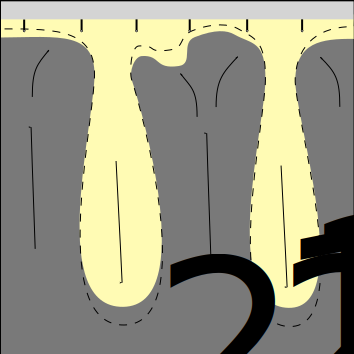
\includegraphics[width=9cm]{./plot/Konvektion_Diffusion.pdf}
 \caption{Interpretation der auftretenden Phänomene, verursacht durch Konvektion und Diffusion}
 \label{fig:difkon}
\end{figure}
% 
% \centering
% 
% \graph[./plot/Konvektion_Diffusion.pdf]{Interpretation der auftretenden Phänomene, verursacht durch Konvektion und Diffusion}{fig:difkon}

\twocolumn

% \newpage
% \mbox{\,}
% \newpage

\section{\COTm Experiment mit porösem Medium}
\label{res:cpm}

\graph[./plot/BCG_test_03_num]{Farbumschläge des \BCG in Verbindung mit verschiedenen Substanzen. \BCG (1) in neutraler Form, \dah im Gleichgewicht mit der umgebenden Luft, (2) in Kombination mit \COT. Man kann sehr gut den Ausschlag ins Gelbe erkennen. (3) mit den Glaskügelchen verschiedener Größen, (4) mit Glaskügelchen und gelöstem \COT.}{fig:CPO}

\graph[./plot/BCG_Test_Boro_num]{Farbumschläge des \BCG. \BCG (1) in neutraler Form, \dah im Gleichgewicht mit der umgebenden Luft, (2) in Kombination mit gelöstem \COT. Man kann sehr gut den Ausschlag ins Gelbe erkennen. (3) mit den Glaskügelchen aus Borosilikatglas, (4) mit Glaskügelchen und gelöstem \COT.}{fig:CPO_bor}

Der Versuch das \COT Experiment in Kombination mit einem porösen Medium durchzuführen ist aufgrund der verwendeten Glaskugeln gescheitert. Es wurde nicht beachtet, dass Glas Wasser durch Ionenaustausch basisch macht. Die leicht löslichen Elemente an der Oberfläche des Glases werden vom Wasser herausgelöst und durch die im Wasser vorhandenen H$^+$-Ionen ersetzt. Dadurch wird das Wasser basisch, da die OH$^-$-Konzentration steigt. \citep{Vogel}

Dieser Effekt ist durch die große Oberfläche, die die Kügelchen insgesamt haben, nicht zu vernachlässigen und sorgt dafür, dass der benutze Indikator nur den basischen Farbton annimmt. Das Lösen von \COT im Wasser kann diesen Effekt offensichtlich nicht überwiegen.

Zur Verdeutlichung der beschriebenen Phänomene siehe Abbildung \ref{fig:CPO}.

Ein angedachter Lösungsansatz mit Glaskugeln, welche dem Wasser gegenüber beständiger sind, wurde aus Zeitgründen nicht umgesetzt. Ein Test der Kugeln aus Borosilikatglas ergab aber vielversprechende Ergebnisse, da der durch das \COT hervorgerufene Farbumschlag auch mit Kugeln in der Indikatorlösung beobachtet werden konnte. Siehe dazu Abbildung \ref{fig:CPO_bor}.

% \vspace{10cm} % damit balance die Bilder beide auf die Seite packt



  
% ========================= longgraphpages =========================
\longgraphpage[./plot/plots_data-1/plot_all_overview_quot_0]{Fingerbildung Experiment 1. Die Farbskala beschreibt die relative Absorption im Bezug auf den Hintergrund (0). Maximale Absorption bekommt den Wert 100 zugewiesen.}{fig:vcot_1-1}
\longgraphpage[./plot/plots_data-1/plot_all_overview_quot_1]{Fingerbildung Experiment 1. Die Farbskala beschreibt die relative Absorption im Bezug auf den Hintergrund (0). Maximale Absorption bekommt den Wert 100 zugewiesen.}{fig:vcot_1-2}

\longgraphpage[./plot/plots_data-1/finger_detection_cut]{Abgebildet sind Fingerbildung zusammen mit detektierten Fingerpositionen und -längen zur Demonstration, wie die in Teil \ref{sec:lan} beschriebene Methode funktioniert. Die Farbskala beschreibt die relative Absorption im Bezug auf den Hintergrund (0). Maximale Absorption bekommt den Wert 100 zugewiesen.}{fig:f_detect}


\longgraphpage[./plot/plots_data-1/plot_all_overview_0_adj]{Fingerbildung Experiment 1. Rohaufnahmen mit erhöhtem Kontrast. Zu erkennen ist der Übergang vom diffusiven zum konvektiven Prozess nach ca. \SI{9}{\minute}. Auch kann man beobachten, wie die diffusive Schicht zwischen den Fingern ``abgesaugt'' wird. }{fig:vcot_1-grey}
% ========================= einzelner Finger =========================
\longgraphpagetriple{./plot/plots_data-1/single_evolution_1}{./plot/plots_data-1/single_evolution_2}{./plot/plots_data-1/single_evolution_3}{Entwicklung eines einzelnen Fingers mit der Zeit.}{fig:sevo}

\longgraphpagesextuple{./plot/plots_data-1/comp_evolution_1}{./plot/plots_data-1/comp_evolution_2}{./plot/plots_data-1/comp_evolution_3}{./plot/plots_data-1/comp_evolution_4}{./plot/plots_data-1/comp_evolution_5}{./plot/plots_data-1/comp_evolution_6}{Überblick über den gesamten Verlauf des Experiments}{fig:complete}
% \widegraphpage[./plot/plots_data-1/fingers_quot-raw_5-30_cut.png]{Vergleich der Quotientenmethode und dem tatsächlich aufgezeichneten Bild.}{fig:fing_comp}


% \chapter{Ausblick}
% \input{./docu/06_Schlussfolgerungen}

\chapter{Zusammenfassung}

\label{cha:con}

In dieser Arbeit wurde gezeigt, wie sich durch das Lösen von \COT in Wasser Dichteinstbilitäten ausbilden, welche zu Fingerbildung und damit \COT-Sequestration führen. Die Beobachtungen wurden ausführlich beschrieben und versucht zu deuten.
Die Experimente wurden in einer \HSC durchgeführt, die für eine prinzipiell zweidimensionale Versuchanordnung sorgt und mit einer Kamera gefilmt.
Mit Hilfe von Python wurden die Bilder ausgewertet und die gewonnen Daten geplottet.
Die Auswertungen lassen erkennen, dass sich das Experiment in drei Phasen gliedert:
\begin{itemize}
 \item Diffusion (\SI{0}{\minute} bis \SI{9}{\minute})
 \item stabile Fingerbildung (\SI{9}{\minute} bis \SI{60}{\minute})
 \item Turbulenz (\SI{60}{\minute} bis zum Ende) 
\end{itemize}


Ein Versuch das Experiment mit einem porösen Medium durchzuführen ist fehlgeschlagen. Es konnten aber wertvolle Informationen für kommende Versuche dieser Art gewonnen werden. So waren Kugeln aus \KNG ungeeignet für das Experiment, da sie das Wasser basisch machen, wodurch eine Beobachtung der \COT Bewegung mit Hilfe des \BCG-Indikators unmöglich war. Kugeln aus \BOG hingegen schienen den Indikator nicht so stark zu beeinflussen.

\section{Ausblick}
\begin{itemize}
 \item Poröses Medium
 \item Methoden verbessern
 \item verschieden dicke \HSCs $\Rightarrow$ verschiedene $Ra$
\end{itemize}


\onecolumn
\bibliographystyle{plainnat}
% \citestyle{egu}
\bibliography{./docu/bibliography}

\onecolumn

\chapter*{Erkl\"{a}rung}

Ich versichere, dass ich diese Arbeit selbstst\"{a}ndig verfasst und keine anderen als die angegebenen Quellen und Hilfsmittel benutzt habe.

\vspace{2cm}

Heidelberg, den 1.April 2015,

%Unterschrift % von der Uni gefordert. ggf anpassen
\end{document}
